\subsection{Qué sí cubre la literatura revisada}

Los catorce papers, leídos en cruz y no eje por eje, dejan esto:

\begin{enumerate}
  \item OpenAPI es el formato con el que se especifica REST (E1). Casas et al.\ (2021) lo muestran
        en 47 artículos; Mainas et al.\ (2023) prueban que se puede enriquecer semánticamente sobre
        corpus reales.
  \item Hay marcos para cruzar esquemas (E2) y para medir significado (E3). Shvaiko y Euzenat
        (2005) y El Bayadh et al.\ (2015) se pueden reutilizar; Santos Sousa et al.\ (2026) ya
        documentaron dónde fallan los \textit{embeddings}.
  \item E4 separa dominio e interfaz. Schmidt y Thiry (2020) hablan de microservicios; BIAN juega
        el mismo papel como referencia de capacidad.
  \item E5 es otro oficio. Ehsan et al.\ (2022) y Golmohammadi et al.\ (2024) usan OpenAPI para
        probar APIs vivas. Eso recorta el plan: calidad operativa $\neq$ coherencia con BIAN.
  \item E6 (Mahanra Rao et al., 2025) rankea servicios por QoS. Consume descripciones; no pregunta
        si el YAML bancario refleja un \ServiceDomain{}.
\end{enumerate}

La pregunta del grupo sigue sin respuesta en ese corpus: \textit{¿en qué medida un contrato
OpenAPI bancario refleja un \ServiceDomain{} BIAN, y cómo se puntúa eso de modo que otro pueda
repetirlo?}

\subsection{Vacíos identificados}

\begin{table}[H]
  \centering
  \caption{Vacíos identificados en la literatura (V1--V5)}
  \label{tab:vacios}
  \small
  \begin{tabular}{@{}p{0.14\textwidth}p{0.38\textwidth}p{0.38\textwidth}@{}}
    \toprule
    \textbf{Vacío} & \textbf{Evidencia en el review} & \textbf{Implicación para la tesis} \\
    \midrule
    \textbf{V1 --- Intersección OpenAPI $\cap$ BIAN} &
    Ningún paper del corpus junta ambos artefactos en banca &
    Objeto: contrato OpenAPI vs.\ SD BIAN \\
    \textbf{V2 --- Métrica integrada} &
    E2 y E3 dan técnicas sueltas; E1 no mide alineación &
    Producto: S, E, C y \AlignmentScore{} \\
    \textbf{V3 --- Cobertura de conceptos} &
    La cobertura ontológica no se calcula sobre \BusinessObject{} BIAN en OpenAPI &
    \CoverageScore{} \\
    \textbf{V4 --- Procedimiento reproducible} &
    Mainas et al.\ (2023): RDF, sin score ni nivel &
    Diseño del Cap.~4 \\
    \textbf{V5 --- Gobernanza documental} &
    E5 y E6: \textit{runtime} o ranking, no deriva contrato--modelo &
    Medir antes del despliegue \\
    \bottomrule
  \end{tabular}
\end{table}


La \Cref{fig:brecha} pasa de E1--E6 a los vacíos V1--V5.

\begin{figure}[H]
  \centering
  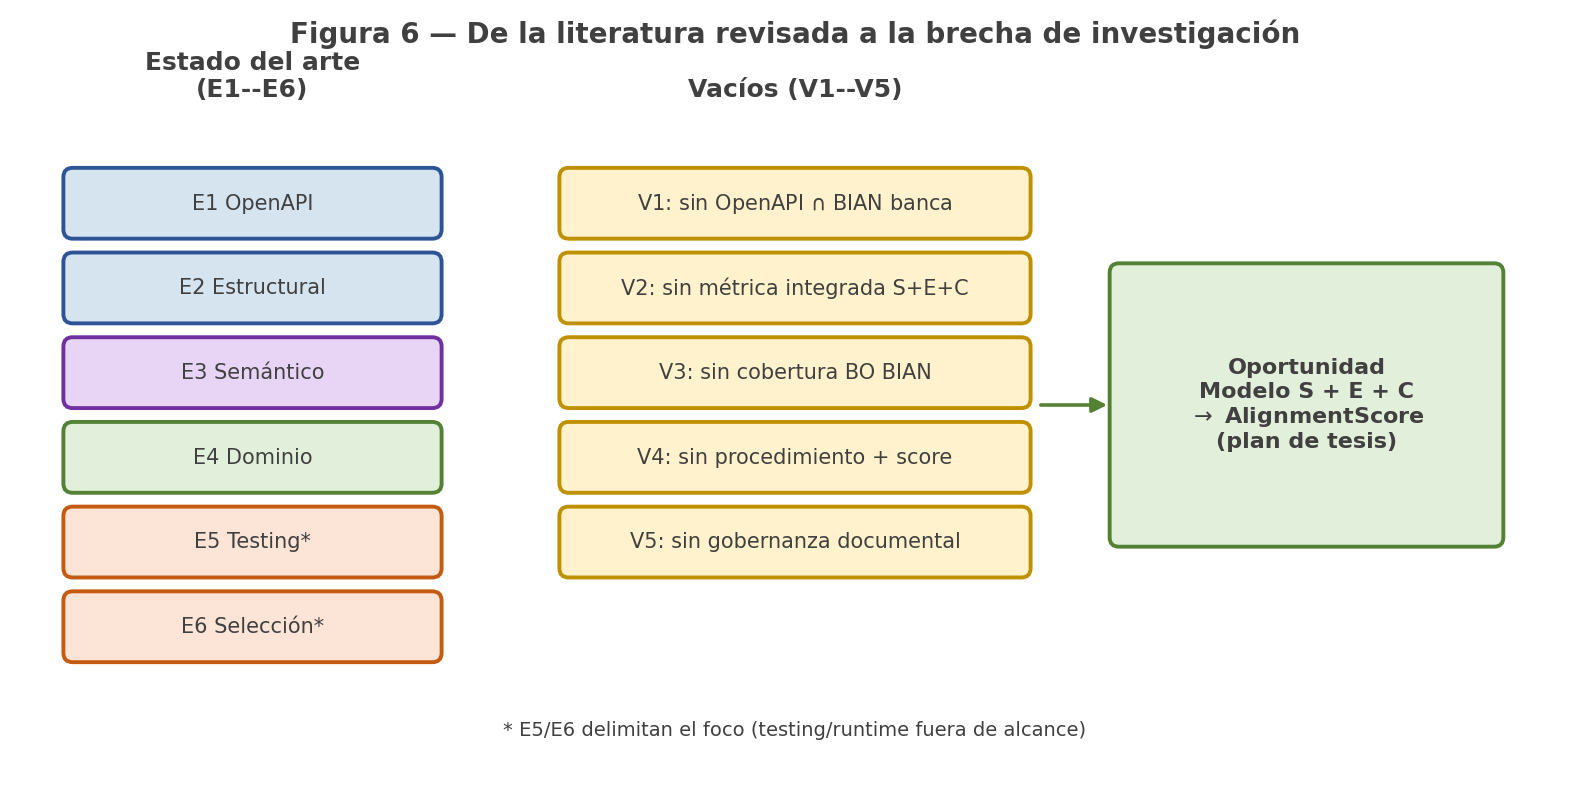
\includegraphics[width=0.95\textwidth]{Figura_06_Brecha}
  \caption{De la literatura revisada (E1--E6) a la brecha de investigación (V1--V5)}
  \label{fig:brecha}
\end{figure}

\subsection{Oportunidad de investigación}

Cinco fases. Primera: escribir el modelo. Luego OE1 (normalizar), OE2--OE3 (E y S; C junto a
OE4) y el \AlignmentScore{} con umbrales Alta / Media / Baja / Nula.

Guía~1 se queda en el papel (\Cref{sec:alcances}). Cubre V1--V4 sobre documentos. No cubre
testing (E5) ni un sello de cumplimiento.
